\documentclass[a4paper,11pt]{report}
%\pagestyle{headings}

% des paquetages indispensables, qui ajoutent des fonctionnalites
%\usepackage[latin1]{inputenc}
\usepackage[utf8]{inputenc}
\usepackage[french]{babel}
%\usepackage{lmodern}
\usepackage{amsmath,amssymb}
\usepackage{amsthm}
\usepackage{fullpage}
\usepackage{graphicx}
\usepackage{url}
\usepackage{xspace}
\usepackage{listings}
\usepackage{xcolor}
\usepackage{hyperref}
\usepackage{eurosym}

%%configuration de listings pour l'affichage du code
%\lstset{
%    language=C,
%    basicstyle=\ttfamily\small, %
%    identifierstyle=\color{red}, %
%    keywordstyle=\color{blue}, %
%    stringstyle=\color{black!60}, %
%    commentstyle=\it\color{black!50}, %
%    columns=flexible, %
%    tabsize=3, %
%    extendedchars=true, %
%    showspaces=false, %
%    showstringspaces=false, %
%    numbers=left, %
%    numberstyle=\tiny, %
%    breaklines=true, %
%    breakautoindent=true, %
%    captionpos=b,
%    frame=single
%}

% On fera des listes a puce et non a tiret.
\renewcommand{\FrenchLabelItem}{\textbullet}

\newtheorem{theoreme}{Th\'{e}or\`{e}me}
\newtheorem{definition}{D\'{e}finition}
\newtheorem{exercice}{Exercice}

\newcommand{\tab}{\hspace*{\parindent}}

%Definition de quelques commandes utiles en maths :

% R et N
\newcommand{\R}{\mathbb{R}}
\newcommand{\N}{\mathbb{N}}
\newcommand{\C}{\mathbb{C}}
% derive partielle et congruence
\newcommand{\drond}{\partial}
\newcommand{\congru}{\equiv}
% blocs parenthese, valeur absolue, norme, crochets, accolades
\newcommand{\abs}[1]{\left\lvert#1\right\rvert}
\newcommand{\norm}[1]{\left\lVert#1\right\lVert}
\newcommand{\braces}[1]{\left(#1\right)}
\newcommand{\croch}[1]{\left[#1\right]}
\newcommand{\cbraces}[1]{\left\{#1\right\}}
% blocs parties entieres superieur et inferieur
\newcommand{\entsup}[1]{\left\lceil#1\right\rceil}
\newcommand{\entinf}[1]{\left\lfloor#1\right\rfloor}





\title{Cannonball of RC cars\\User guide}
\author{Thibaut Coutelou, Benjamin Mugnier, Guillaume Perrin}
\date{\today}

\begin{document}
\maketitle
\tableofcontents
%\listoffigures

\setlength{\parskip}{3mm}

%\begin{figure}[!ht]
%\begin{center}
%\includegraphics[width=\textwidth]{img/acteurs}
%\caption{Acteurs}
%\label{acteurs}
%\end{center}
%\end{figure}

%Quick reminder of latex :
%part
%chapter
%section
%subsection
%subsubsection
%paragraph

%Don't forget : set ts=79







\chapter{Quick starter guide}

\section{What do I need ?}

\section{How to plug ?}

Follow instructions on figure \ref{fig:wires}.

\begin{figure}[!ht]
\centering
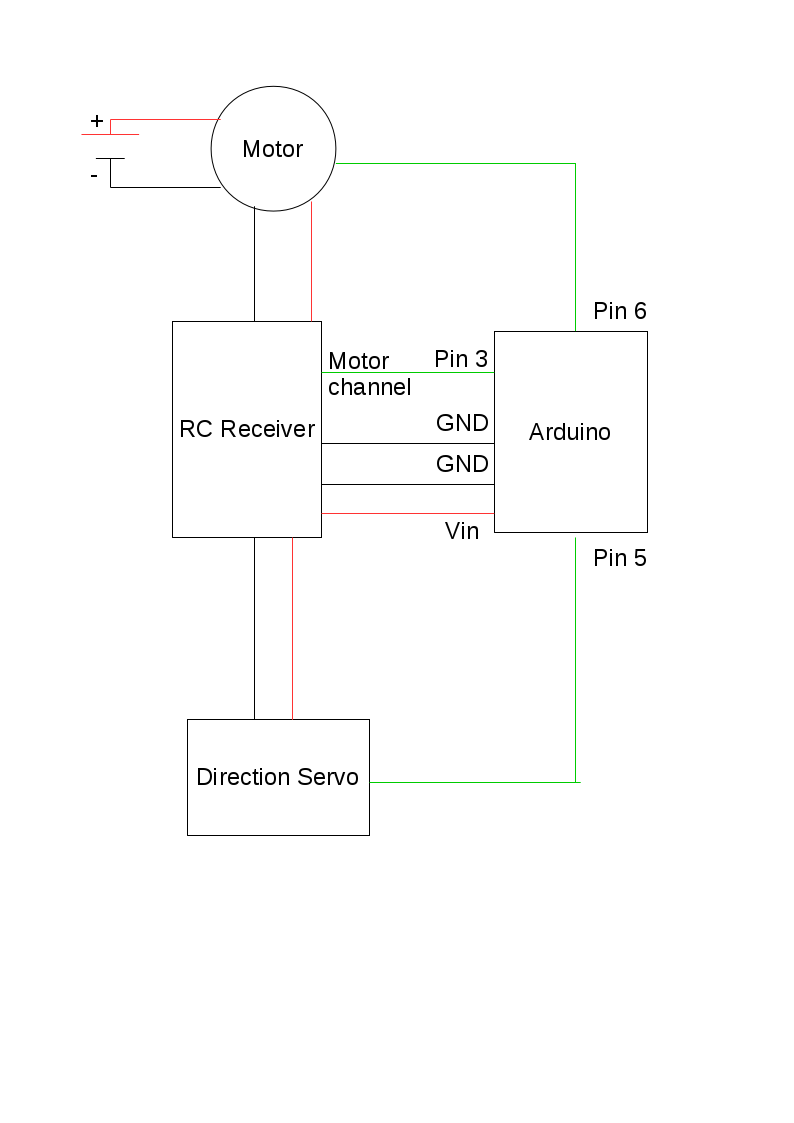
\includegraphics[scale=0.5]{img_static/wires}
\caption{How to plug}
\label{fig:wires}
\end{figure}

\section{How to build the program ?}

\section{How to flash the Arduino ?}

There are two ways to flash the Arduino, the first one (and the simple one) is
to use the Arduino IDE\footnote{\url{http://arduino.cc/en/Main/Software\#toc1}}. After
download it, then open the project in.

In order to flash the Arduino, you need to select the model in \texttt{Tools >
Board} and the serial port in \texttt{Tools > Serial Port}, this is likely
\texttt{COM3} or higher on Windows and \texttt{/dev/tty.usbmodem} on Unix systems.
You can now flash the file on Arduino using the shortcut \texttt{upload} or in
the menu \texttt{File > Upload}. You will see \texttt{Upload done} if everything
went well.

If you're interesting of the other method, please refer to \ref{sec:Flashing}.

\section{How to get markers ?}

Marker recognition is based on highly reliable markers (hrm) from the arUco
library.

\subsection{Camera calibration}

First, you need to calibrate the camera. In order to do that, \begin{itemize}

    \item Generate a board of markers with \texttt{aruco\_create\_board 4:5
        boardImageCalibration.png boardConfigurationCalibration.yml}.

    \item Print the png image. Mesure in meters the size of a marker.

    \item Convert the board configuration file from pixel to meters with
        \texttt{aruco\_boar\_pix2meters boardConfigurationCalibration.yml <size
        of marker in meters> boardConfigurationCalibrationMeters.yml}

    \item Calibrate the camera with \texttt{aruco\_calibration live
        boardConfigurationCalibrationMeters.yml cameraParams.yml}

\end{itemize}

\subsection{Creating hrm markers}

You now need to create markers : \begin{itemize}

    \item Generate a dictionary of hrm markers with
        \texttt{aruco\_hrm\_create\_dictionary dict.yml <size of the
        dictionary> <marker size>}

    \item Generate the board with \texttt{aruco\_hrm\_create\_board dict.yml
        board.yml board.png heighr width}

    \item Print the board.

\end{itemize}



\section{How to get metrics ?}

\subsection{Setup a MQTT server}

You need an MQTT server to get the data. We recommend
Mosquitto\footnote{\url{http://mosquitto.org/download/}} which is available for every
platform.  Note that it's available on Debian via a simple \texttt{apt-get install}
mosquitto. As Windows, you need to download the server and then restart your
computer for the service to launch (or ask the service to launch manually),
this is really important.

Then, you need the tablet to be on the same network as the server. You can
either create an hotspot via the tablet or the server, or connect both to an
existing network.  You need to tell the program the server's ip. Please refer
to the corresponding section.

\subsection{Display metrics in HTML}


\section{How to launch the program ?}

\subsection{Arguments needed}







\chapter{User guide}

\section{Building}

\section{Flashing}
\label{sec:Flashing} %Need in user quick guide->flash arduino

\section{Plugging}

\section{Markers}

\section{Monitoring}

\section{Implementing a new artificial intelligence}

\section{Android}

\end{document}
